%%%%%%%%%%%%%%%%%%%%%%%%%%%%%%%%%%%
%This is the LaTeX ARTICLE template for RSC journals
%Copyright The Royal Society of Chemistry 2016
%%%%%%%%%%%%%%%%%%%%%%%%%%%%%%%%%%%

\documentclass[twoside,twocolumn,9pt]{article}

\usepackage{tgheros}
\renewcommand{\familydefault}{\sfdefault}

\usepackage{extsizes}
\usepackage[super,sort&compress,comma]{natbib} 
\usepackage[version=3]{mhchem}
\usepackage[left=1.5cm, right=1.5cm, top=1.785cm, bottom=2.0cm]{geometry}
\usepackage{balance}
\usepackage{mathptmx}
\usepackage{sectsty}
\usepackage{graphicx}
\usepackage{subcaption}
\usepackage{lastpage}
\usepackage[format=plain,justification=justified,singlelinecheck=false,font={stretch=1.125,small,sf},labelfont=bf,labelsep=space]{caption}
\usepackage{float}
\usepackage{fancyhdr}
\usepackage{fnpos}
\usepackage[english]{babel}
\addto{\captionsenglish}{%
  \renewcommand{\refname}{Notes and references}
}
\usepackage{array}
\usepackage{droidsans}
\usepackage{charter}
\usepackage[T1]{fontenc}
\usepackage[usenames,dvipsnames]{xcolor}
\usepackage{setspace}
\usepackage[compact]{titlesec}
\usepackage[utf8]{inputenc}

%%%Please don't disable any packages in the preamble, as this may cause the template to display incorrectly.%%%


\usepackage{xcolor}
\definecolor{ugent_blue}{RGB}{30, 100, 200}
\definecolor{ugent_yellow}{cmyk}{.0, .10, 1, 0}

\usepackage{titlesec}
\titleformat{\section}
{\color{ugent_blue}\normalfont\Large\bfseries}
{\color{ugent_blue}\thesection}{1em}{}

\usepackage[colorlinks=true,linkcolor=black,citecolor=ugent_blue]{hyperref}

\usepackage{lineno}
\linenumbers

\usepackage{hyperref}

%\AtEveryCite{\color{ugent_blue}}




\usepackage{epstopdf}%This line makes .eps figures into .pdf - please comment out if not required.
\usepackage{cleveref}
\definecolor{cream}{RGB}{222,217,201}

%%%package for drawing quantum circuits%%%
\usepackage{tikz}
% TikZ libraries `calc` needed now to tweak bracket.
\usetikzlibrary{backgrounds,fit,decorations.pathreplacing,calc}
% Dirac Kets
\newcommand{\ket}[1]{\ensuremath{\left|#1\right\rangle}}
% package for lines with three dots
\usetikzlibrary{decorations.markings}

% fractions without a line
\usepackage{amsmath}

% complex numbers symbol
\usepackage{amssymb}

\begin{document}

\pagestyle{fancy}
\thispagestyle{plain}
\fancypagestyle{plain}{
%%%HEADER%%%
\renewcommand{\headrulewidth}{0pt}
}
%%%END OF HEADER%%%

%%%PAGE SETUP - Please do not change any commands within this section%%%
\makeFNbottom
\makeatletter
\renewcommand\LARGE{\@setfontsize\LARGE{15pt}{17}}
\renewcommand\Large{\@setfontsize\Large{12pt}{14}}
\renewcommand\large{\@setfontsize\large{10pt}{12}}
\renewcommand\footnotesize{\@setfontsize\footnotesize{7pt}{10}}
\makeatother

\renewcommand{\thefootnote}{\fnsymbol{footnote}}
\renewcommand\footnoterule{\vspace*{1pt}% 
\color{cream}\hrule width 3.5in height 0.4pt \color{black}\vspace*{5pt}} 
\setcounter{secnumdepth}{5}

\makeatletter 
\renewcommand\@biblabel[1]{#1}            
\renewcommand\@makefntext[1]% 
{\noindent\makebox[0pt][r]{\@thefnmark\,}#1}
\makeatother 
\renewcommand{\figurename}{\small{Fig.}~}
\sectionfont{\sffamily\Large}
\subsectionfont{\normalsize}
\subsubsectionfont{\bf}
\setstretch{1.125} %In particular, please do not alter this line.
\setlength{\skip\footins}{0.8cm}
\setlength{\footnotesep}{0.25cm}
\setlength{\jot}{10pt}
\titlespacing*{\section}{0pt}{4pt}{4pt}
\titlespacing*{\subsection}{0pt}{15pt}{1pt}
%%%END OF PAGE SETUP%%%

%%%FOOTER%%%
\fancyfoot{}
\fancyfoot[LO,RE]{\vspace{-7.1pt}
\includegraphics[height=9pt]{head_foot/LF}}
\fancyfoot[CO]{\vspace{-7.1pt}\hspace{11.9cm}
\includegraphics{head_foot/RF}}
\fancyfoot[CE]{\vspace{-7.2pt}\hspace{-13.2cm}
\includegraphics{head_foot/RF}}
\fancyfoot[RO]{\footnotesize{\sffamily{1--\pageref{LastPage} {\color{ugent_yellow} ~\textbar } \hspace{2pt}\thepage}}}
\fancyfoot[LE]{\footnotesize{\sffamily{\thepage~{\color{ugent_yellow} ~\textbar }\hspace{4.65cm} 1--\pageref{LastPage}}}}
\fancyhead{}
\renewcommand{\headrulewidth}{0pt} 
\renewcommand{\footrulewidth}{0pt}
\setlength{\arrayrulewidth}{1pt}
\setlength{\columnsep}{6.5mm}
\setlength\bibsep{1pt}
%%%END OF FOOTER%%%

%%%FIGURE SETUP - please do not change any commands within this section%%%
\makeatletter 
\newlength{\figrulesep} 
\setlength{\figrulesep}{0.5\textfloatsep} 

\newcommand{\topfigrule}{\vspace*{-1pt}% 
\noindent{\color{cream}\rule[-\figrulesep]{\columnwidth}{1.5pt}} }

\newcommand{\botfigrule}{\vspace*{-2pt}% 
\noindent{\color{cream}\rule[\figrulesep]{\columnwidth}{1.5pt}} }

\newcommand{\dblfigrule}{\vspace*{-1pt}% 
\noindent{\color{cream}\rule[-\figrulesep]{\textwidth}{1.5pt}} }

\makeatother
%%%END OF FIGURE SETUP%%%

%%%TITLE, AUTHORS AND ABSTRACT%%%
\twocolumn[
  \begin{@twocolumnfalse}
{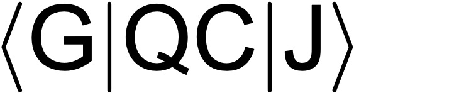
\includegraphics[height=30pt]{head_foot/journal_name}\hfill\raisebox{0pt}[0pt][0pt]{
\includegraphics[height=55pt]{head_foot/RSC_LOGO_CMYK}}\\[1ex]

\includegraphics[width=18.5cm]{head_foot/header_bar}}\par
\vspace{1em}
\sffamily
\begin{tabular}{m{4.5cm} p{13.5cm} }

& \noindent\LARGE{\textbf{Implementing Unitary Coupled Cluster On a Quantum Computer$^\dag$}} \\%Article title goes here instead of the text "This is the title"
\vspace{0.3cm} & \vspace{0.3cm} \\

& \noindent\large{Oskar Grzegorowski$^{\ast}$\textit{$^{a}$}} \\%Author names go here instead of "Full name", etc.

& \\

& \noindent\normalsize{The scaling of classical Unitary Coupled Cluster remains to be one of the biggest hindrances holding the theory back, however its implementations on quantum computers have the potential to solve this issue, and elevate the theory beyond its current limits. That said, to many the construction of UCC ansätze within quantum circuits, and the processes surrounding their applications, remain ambiguous. In this outline we provide an in depth exploration of UCC ansätze and their implementation on quantum computers. We introduce variations of UCC designed specifically with quantum circuits in mind, notably k-UpCCGSD, and compare the performance of their implementations run on both ideal, and currently available noisy quantum devices. Our findings demonstrate that in theory quantum computing can enhance UCC capabilities, however its practical implementations are held back by the severe limitations of modern quantum computers.} \\
% This article provides an in-depth exploration of Unitary Coupled Cluster (UCC), its integration into quantum circuits, and the necessary basics of quantum computing. Additionally we introduce alternative versions of UCC, designed to increase the accuracy and efficiency of standard implementations, notably the k-UpCCGSD ansatz.
% The latter sections of the article present and discuss dissociation curves of $\text{H}_2$ obtained using custom ansätze and run on both ideal and noisy quantum backend simulations.
% Throughout this article, our aim is to provide a comprehensive outlook on UCC from the perspective of quantum computing, and the potential advancements it could lead to in the field of computational chemistry
\end{tabular}

\end{@twocolumnfalse} \vspace{1.6cm}

]
%%%END OF TITLE, AUTHORS AND ABSTRACT%%%

%%%FONT SETUP - please do not change any commands within this section
\renewcommand*\rmdefault{bch}\normalfont\upshape
\rmfamily
\section*{}
\vspace{-1cm}


% %%%FOOTNOTES%%%

\footnotetext{\textit{$^{a}$Corresponding author: Oskar.Grzegorowski@UGent.be}}

% %Please use \dag to cite the ESI in the main text of the article.
% %If you article does not have ESI please remove the the \dag symbol from the title and the footnotetext below.
% \footnotetext{\dag~Electronic Supplementary Information (ESI) available: [details of any supplementary information available should be included here]. See DOI: 00.0000/00000000.}
% %additional addresses can be cited as above using the lower-case letters, c, d, e... If all authors are from the same address, no letter is required

% \footnotetext{\ddag~Additional footnotes to the title and authors can be included \textit{e.g.}\ `Present address:' or `These authors contributed equally to this work' as above using the symbols: \ddag, \textsection, and \P. Please place the appropriate symbol next to the author's name and include a \texttt{\textbackslash footnotetext} entry in the the correct place in the list.}


%%%END OF FOOTNOTES%%%

%%%MAIN TEXT%%%%


\section{Introduction}
Quantum computing remains to be one of the most promising ways of advancing the way we understand and simulate molecular systems. In theory, it should allow us to go beyond the scope of classical machines, and develop new innovative tools which open up new avenues in the field of computational quantum chemistry. Due to their quantum nature, quantum computers excel in many areas where classical computers struggle, such as simulating quantum systems or solving certain types of optimization problems. Among the various quantum inspired approaches, the application of quantum computing principles into Unitary Coupled Cluster Theory stands out as a compelling approach to advancing the accuracy and efficiency of CC calculations.

Coupled Cluster Theory stands as a powerful and widely used method for accurately describing the structure and properties of many-body systems. However, the traditional classical implementations of UCC are often hindered by their exponential scaling with system size, which renders its application to larger molecules limited. Quantum computers have the potential to handle larger systems more efficiently, allowing UCC to tackle problems currently beyond the reach of classical CC.

It is however important to note, that while in theory a quantum implementation of UCC has the capacity to outperform its classical counterpart, it would require accurate and robust hardware to operate on. Current quantum computers have made significant strides in terms of their capabilities, but they still face challenges in terms of accuracy. They are highly sensitive devices, extremely prone to noise and errors, which leads to calculational inaccuracies.

\section{Theory}

\subsection{Coupled Cluster Theory}

In quantum chemistry Coupled Cluster (CC) \cite{Anand2022} is a post Hartree-Fock method used to describe the electronic structure of many body systems. It has been used to compute relatively accurate approximations of various molecular properties while being less computationally demanding than methods such as FCI (Full Configuration Interaction). The CC wavefunction is given by a series of excitation operators acting on a reference state, typically a Slater determinant constructed from Hartree-Fock orbitals:

\begin{align}
  |\Psi_{\text{CC}}\rangle = e^{\hat{\text{T}}} |\Phi_{\text{ref}}\rangle
\end{align}

here $|\Phi_{\text{ref}}\rangle$ is the HF reference state, and operator $\hat{\text{T}}$ is the cluster operator. The choice of cluster operator, in conjunction with a strategy for determining the optimal amplitudes described below, defines a given method, and the general form of the state created by the application of the cluster operator is called an ansatz. If this operator consists of fermionic excitations from occupied to virtual orbitals, the generated ansatz is referred to as traditional coupled-cluster (TCC), and its exponential map is given by its Taylor expansion:

\begin{align}
\hat{\text{T}}=\sum_{k=1}^n\hat{\text{T}}_k
\end{align}
\begin{align}
  \hat{\text{T}}_k = \frac{1}{(k\text{!})^2} \sum_{\genfrac{}{}{0pt}{}{i,j,...}{a,b,...}}t^{ab\ldots{}}_{ij\ldots{}}\hat{\text{a}}^{\dagger}_a\hat{\text{a}}^{\dagger}_b\ldots{}\hat{\text{a}}_j\hat{\text{a}}_i
\end{align}

here each $\hat{\text{T}}_n$ consists of $k$ annihilation and $k$ creation operators acting on occupied and virtual orbitals in the reference state respectively. The choice of different values of n yields different truncated ansätze. If n equals the number of electrons, the FCI wave function lies within the manifold of wavefunctions represented by the TCC wave function and no approximation is made.
Comparing the exact CC solution with full CI, where each $\hat{C}_i$ is the operator which generates all $i$-fold configuration terms, it can be shown that \cite{Bartlett2007}:

  \begin{flalign}
    & \hat{C}_1=\hat{T}_1 \\
    & \hat{C}_2=\hat{T}_2+\frac{1}{2}\hat{T}_1^2 \\
    & \hat{C}_3=\hat{T}_3+\hat{T}_1\hat{T}_2+\frac{1}{3!}\hat{T}_1^3 \\
    & \hat{C}_4=\hat{T}_4+\frac{1}{2}\hat{T}_2^2+\hat{T}_1\hat{T}_3+\frac{1}{2}\hat{T}_1^2\hat{T}_2+\frac{1}{4!}\hat{T}_1^3
    \end{flalign}

In these decompositions it can be seen that for a given $i$-fold configuration term, all $\hat{T}_j$ terms for $j \leq i$ are contributing to the expression for the operator. Hence for example, a coupled-cluster wave function limited to only double excitations already includes the disconnected parts of quadruples, hextuples, and higher even ordered excitations. This implicit connection to all higher order configurations grants truncated CC and its variations a considerable degree of accuracy, out-performing essentially all other standard single-reference methods with comparable computational cost.

\subsection{Basics of Quantum Computing}

This section contains the basics of quantum computing theory necessary for understanding the contents of this outline.
In quantum computing (QC) \cite{Silva2023} quantum-mechanical phenomena such as superposition and entanglement, are used to process information. In QC, the basic unit of information is the qubit, which, unlike classical bits, which have to be in state 0 or 1, can exist in a superposition, a linear combination of states with complex coefficients or amplitudes. The modulus square of each amplitude is the probability of the corresponding state being observed, and the sum of the modulus square of all possible states must equal to 1. This result is known as the Born's rule. For a two-level qubit defined in the orthonormal basis, state 0 or 1 can be represented as unit vectors:

\begin{align}
|0\rangle=\dbinom{1}{0} \quad\text{and}\quad |1\rangle=\dbinom{0}{1}
\end{align}

In this instance the superposition between the two states can be represented as:

\begin{align}
  |\Psi\rangle = \alpha|0\rangle + \beta|1\rangle, \quad \text{where } \alpha, \beta \in \mathbb{C}
\end{align}

In quantum mechanics an operator is unitary if its Hermitian conjugate is equal to its inverse:

\begin{align}
\hat{U}^{\dagger}=\hat{U}^{-1}
\end{align}

and the operator multiplied by its Hermitian conjugate gives the identity operator:

\begin{align}
  \hat{U}^{\dagger}\cdot\hat{U}=\hat{U}\cdot\hat{U}^{\dagger}=\hat{I}
  \end{align}

In QC it is necessary that any operators acting on qubits are unitary. When an operation is applied to a quantum state, the probabilities of different measurement outcomes should still add up to 1 (the sum of the modulus square of all possible states must equal to 1). Unitary operators ensure that the total probability remains conserved. Another reason is that unitary operators are reversible, meaning that they can be applied in both the forward and backward directions, which allows for manipulation and transformation of quantum states without losing any information. In quantum computing, unitary operators can be represented as matrices, and they are commonly referred to as gates. Unitary gates acting on qubits are fundamental building blocks in quantum circuits.
Here is a short list of fundamental quantum gates used in this outline:\\
Pauli matrices:

\begin{equation}
  \begin{split}
    \sigma_0\equiv I=\begin{pmatrix}
      1 & 0 \\
      0 & 1
    \end{pmatrix} \quad&\quad
    \sigma_1\equiv\sigma_x\equiv X=\begin{pmatrix}
      0 & 1 \\
      1 & 0
    \end{pmatrix} \\
    \sigma_2\equiv\sigma_y\equiv Y=\begin{pmatrix}
      0 & -i \\
      i & 0
    \end{pmatrix} \quad&\quad
    \sigma_3\equiv\sigma_z\equiv Z=\begin{pmatrix}
      1 & 0 \\
      0 & -1
    \end{pmatrix}
  \end{split}
  \end{equation}

These gates act on qubits, and allow to reach any point in the geometrical representation called the Bloch sphere \cref{fig:block}, where a qubit is represented as a point on a sphere. A commonly adopted convention designates the two antipodal points on the sphere as representatives of the computational basis elements.

\begin{center}
  \begin{figure}
      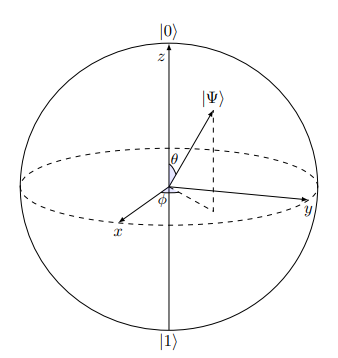
\includegraphics[width=\linewidth]{block_sphere.png}
      \caption{Taken from: \cite{Silva2023}; Exemplary drawing of a block sphere. A Bloch sphere is a geometric representation of the state space of a single qubit in quantum computing, visualizing the possible quantum states as points on a unit sphere. In this example three qubits are shown: qubit $|0\rangle$ is in state 0 (off), qubit $|1\rangle$ is in state 1 (on), and qubit $|\Psi\rangle$ is a superposition between states $|0\rangle$ and $|1\rangle$.}
      \label{fig:block} 
  \end{figure}
\end{center}

The $X$ gate is also called the $NOT$ gate, as it flips the basis set of a qubit ($|0\rangle\rightarrow|1\rangle,\quad|1\rangle\rightarrow|0\rangle$).\\
The Hadamard gate is one of the most important single qubit gates. It enables to put a qubit from a definite computational basis state into a superposition of the two states:

\begin{align}
  H=\frac{1}{\sqrt[]{2}}\begin{pmatrix}
    1 & 1 \\
    1 & -1
  \end{pmatrix}
\end{align}

When applied to $|0\rangle$ and $|1\rangle$ it returns:

\begin{equation}
  \begin{split}
  H|0\rangle=\frac{1}{\sqrt[]{2}}\begin{pmatrix}
    1 & 1 \\
    1 & -1
  \end{pmatrix}\dbinom{1}{0}=\frac{1}{\sqrt[]{2}}\dbinom{1}{1}=\frac{1}{\sqrt[]{2}}|0\rangle+\frac{1}{\sqrt[]{2}}|1\rangle
  \\
  H|1\rangle=\frac{1}{\sqrt[]{2}}\begin{pmatrix}
    1 & 1 \\
    1 & -1
  \end{pmatrix}\dbinom{0}{1}=\frac{1}{\sqrt[]{2}}\dbinom{1}{-1}=\frac{1}{\sqrt[]{2}}|0\rangle-\frac{1}{\sqrt[]{2}}|1\rangle
  \end{split}
  \end{equation}

The total probability of the resulting states (the sum of squares of absolute amplitudes associated with each basis state, or the length of the vector connecting the origin to the point represented by the qubit on a block sphere) is in both cases equal 1, which means that Born's rule is satisfied and if we perform a measurement, there is an equal probability 0.5 of measuring either state $|0\rangle$ or $|1\rangle$. On the block sphere, the Hadamard gate can be understood as a rotation of 180\textsuperscript{o} around the x and z axes.


The $R_x(\theta)$ gate is a gate performing a rotation around the x axis, where $\theta$ is the rotation angle:

\begin{equation}
  R_x(\theta) = \begin{pmatrix}
  \cos\frac{\theta}{2} & -i\sin\frac{\theta}{2} \\
  -i\sin\frac{\theta}{2} & \cos\frac{\theta}{2}
  \end{pmatrix}
\end{equation}
Analogously the $R_z(\theta)$ gate is a gate performing a rotation around the z-axis, where $\theta$ is the rotation angle:
\begin{equation}
  R_z(\theta) = \begin{pmatrix}
  e^{-i\frac{\theta}{2}} & 0 \\
  0 & e^{i\frac{\theta}{2}}
  \end{pmatrix}
\end{equation}

Another main gate, but acting on two qubits, is the controlled-NOT $CNOT$ gate, defined as:

\begin{equation}
CNOT=\begin{pmatrix}
  1 & 0 & 0 & 0 \\
  0 & 1 & 0 & 0 \\
  0 & 0 & 0 & 1 \\
  0 & 0 & 1 & 0 \\
\end{pmatrix}
\end{equation}

This gate is used to entangle two single qubits.
Here is an example of a quantum circuit containing a $CNOT$ gate \href{https://algassert.com/quirk#circuit={%22cols%22:[[%22%E2%80%A2%22,%22X%22]],%22init%22:[1]}}{[see in a simulator]}:

\begin{center}
\begin{tikzpicture}[thick]
    % `operator' will only be used by Hadamard (H) gates here.
    % `phase' is used for controlled phase gates (dots).
    % `surround' is used for the background box.
    \tikzstyle{operator} = [draw,fill=white,minimum size=1.5em] 
    \tikzstyle{phase} = [draw,fill,shape=circle,minimum size=5pt,inner sep=0pt]
    \tikzstyle{not} = [font=\bfseries,draw,shape=circle,minimum size=5pt,inner sep=0pt]
    \tikzstyle{surround} = [fill=blue!15,thick,draw=black,rounded corners=2mm,inner ysep=7pt]
    %
    \matrix[row sep=0.4cm, column sep=0.2cm] (circuit) {
    % First row.
    \node (q1) {$q_0$}; &&
    \node[phase] (P12) {}; &&&
    \coordinate (end1); \\
    % Second row.
    \node (q2) {$q_1$}; &&
    \node[not] (P22) {|}; &&&
    \coordinate (end2);\\
    };
    \begin{pgfonlayer}{background}
        % Draw background box.
        \node[surround] (background) [fit = (q1) (P22) (end2)] {};
        % Draw lines.
        \draw[thick] (q1) -- (end1)  (q2) -- (end2) (P12) -- (P22);
    \end{pgfonlayer}
    %
    \end{tikzpicture}
  \end{center}

In this example qubit $q_0$ is the control qubit, and the $NOT$ gate is applied to qubit $q_1$ if $q_0$ is in the "on" state $|1\rangle$.\\
In this example a Hadamard gate is applied to $q_0$, which means that a superposition is applied to the control gate \href{https://algassert.com/quirk#circuit={%22cols%22:[[%22Chance%22,%22Chance%22],[%22Bloch%22,%22Bloch%22],[%22H%22],[%22Bloch%22],[%22%E2%80%A2%22,%22X%22]],%22init%22:[1]}}{[see in a simulator]}:

\begin{center}
\begin{tikzpicture}[thick]
  % `operator' will only be used by Hadamard (H) gates here.
  % `phase' is used for controlled phase gates (dots).
  % `surround' is used for the background box.
  \tikzstyle{operator} = [draw,fill=white,minimum size=1.5em] 
  \tikzstyle{phase} = [draw,fill,shape=circle,minimum size=5pt,inner sep=0pt]
  \tikzstyle{not} = [font=\bfseries,draw,shape=circle,minimum size=5pt,inner sep=0pt]
  \tikzstyle{surround} = [fill=blue!15,thick,draw=black,rounded corners=2mm,inner ysep=7pt]
  %
  \matrix[row sep=0.4cm, column sep=0.2cm] (circuit) {
  % First row.
  \node (q1) {$q_0$}; &&
  \node[operator] (H11) {H};&
  \node[phase] (P12) {}; &&&
  \coordinate (end1); \\
  % Second row.
  \node (q2) {$q_1$}; &&&
  \node[not] (P22) {|}; &&&
  \coordinate (end2);\\
  };
  \begin{pgfonlayer}{background}
      % Draw background box.
      \node[surround] (background) [fit = (q1) (P22) (end2)] {};
      % Draw lines.
      \draw[thick] (q1) -- (end1)  (q2) -- (end2) (P12) -- (P22);
  \end{pgfonlayer}
  %
  \end{tikzpicture}
\end{center}

In this case the output on both wires will be a superposition \cref{fig:states}. Once qubits are entangled by a $CNOT$ gate their states become dependent on each other. The qubits can be disentangled by applying another $CNOT$ gate to them.

\begin{center}
  \begin{figure}
      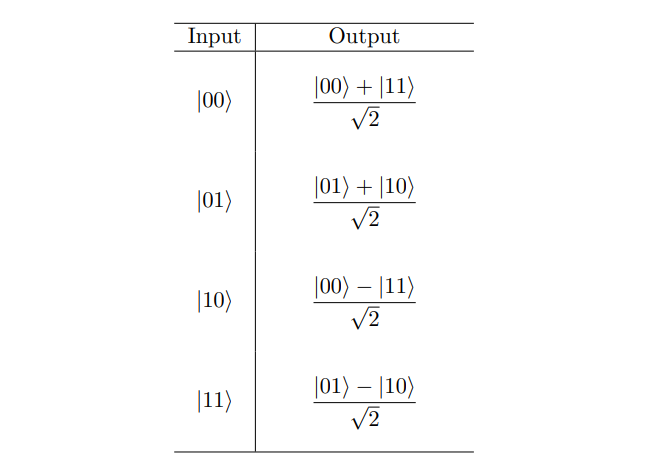
\includegraphics[width=\linewidth]{states_hcnot.png}
      \caption{Taken from: \cite{Silva2023}; The coresponding inputs and outputs on a quantum circuit consisting of a Hadamard gate on the first qubit, and a controlled-NOT gate where the first qubit is the control qubit.}
      \label{fig:states} 
  \end{figure}
\end{center}

\subsection{Implementing the Unitary Coupled Cluster on a Quantum Computer}

Knowing that all operators used in quantum circuits must be unitary, we define Unitary Coupled Cluster \cite{Anand2022} (UCC) as a variation on CC where the cluster operator is of the form $\hat{T}-\hat{T}^{\dagger}$, then $e^{\hat{T}-\hat{T}^{\dagger}}$ is unitary. The cluster operator $\hat{T}$ consists of single, double, ..., (up to $n$-fold) fermionic excitations. On a quantum computer the UCC ansatz is implemented by constructing a unitary operator $U$ defined as such:

\begin{align}
U=e^{\hat{T}-\hat{T}^{\dagger}}
\end{align}
Where the individual excitation operators are given by:
\begin{align}
\hat{T}=\sum\limits_{i}\hat{T}_i
\end{align}

here index $i$ goes over all excitations. In UCC the individual excitation operators do not commute with each other which can lead to complex and non-trivial interactions between them. This makes it challenging to implement UCC in a quantum circuit directly. For this reason approximations have to be done using the Trotter decomposition. The first-order decomposition formula is given by:

\begin{align}
e^{\hat{T}-\hat{T}^{\dagger}}=e^{\sum\limits_{i}\theta_i(\hat{T}_i-\hat{T}_i^{\dagger})}\approx(\prod\limits_{i}e^{\frac{\theta_i}{t}(\hat{T}_i-\hat{T}_i^{\dagger})})^t+O(\frac{1}{t})
\end{align}

where $t$ is the order of decomposition, also called the Trotter number, and $O(\frac{1}{t})$ is the correction term. $\theta_i$ is the amplitude / parameter corresponding to excitation $i$. Using this formula the parameterized wavefunction can be expressed as:

\begin{align}
  |\Psi_{\text{UCC}}(\theta)\rangle=U|\Phi_{\text{ref}}\rangle=e^{\sum\limits_{i}\theta_i(\hat{T}_i-\hat{T}_i^{\dagger})}|\Phi_{\text{ref}}\rangle\approx\\\prod\limits_{i}e^{\theta_i(\hat{T}_i-\hat{T}_i^{\dagger})}|\Phi_{\text{ref}}\rangle
\end{align}

The Trotter decomposition is an approximation, and thus does introduce error, however it is worth noting, that the VQE optimization procedure described later does partially account for the caused error.\\
When individual $\hat{T}_i$ and $-\hat{T}_i^{\dagger}$ terms are put together single and double excitations can be given by \cite{Yordanov2020}:

\begin{align}
  \theta(\hat{T}_p^k-(\hat{T}_p^k)^{\dagger})\equiv\theta(a^{\dagger}_k a_p-a^{\dagger}_p a_k) \quad and\\
  \theta(\hat{T}_{pq}^{kl}-(\hat{T}_{pq}^{kl})^{\dagger})\equiv\theta(a^{\dagger}_k a^{\dagger}_l  a_p a_q - a^{\dagger}_p a^{\dagger}_q a_k a_l)
\end{align}

Unitary operators performing these excitations are then given by:

\begin{align}
U_p^k(\theta)=e^{\theta(\hat{T}_p^k-(\hat{T}_p^k)^{\dagger})} \quad and\\
U_{pq}^{kl}(\theta)=e^{\theta(\hat{T}_{pq}^{kl}-(\hat{T}_{pq}^{kl})^{\dagger})}
\end{align}

These operators can be represented within a quantum circuit by using an encoding such as Jordan-Wigner or Bravyi-Kitaev. Within Jordan-Wigner creation and annihilation operators can be expressed using quantum gates as such:

\begin{align}
a_p=Q_p\prod_{r=0}^{p-1}Z_r=\frac{1}{2}(X_i+iY_i)\prod_{r=0}^{p-1}Z_r \quad and\\
a_p^{\dagger}=Q_p^{\dagger}\prod_{r=0}^{p-1}Z_r=\frac{1}{2}(X_iiY_i)\prod_{r=0}^{p-1}Z_r \quad
\end{align}

where $Q_p=\frac{1}{2}(X_i+iY_i)$ and $Q_p^{\dagger}=\frac{1}{2}(X_iiY_i)$ are the qubit creation and annihilation operators respectively, and $X,Y$ and $Z$ are Pauli matrices. Using these formulas, a single fermionic excitation can be re-expressed using quantum gate operators:

\begin{align}
  U_p^k(\theta)=e^{-i\frac{\theta}{2}(X_pY_k-Y_pX_k)\prod_{r=p+1}^{k-1}Z_r}
\end{align}

Such an exponential of Pauli matrices can be represented as a quantum circuit \cite{Whitfield2011}. To understand the exponential map of the product of Pauli spin matrices, first consider the exponential map of two $Z$ operators. To create the unitary gate $e^{-i\frac{\theta}{2}(Z_0Z_1)}$, a $CNOT$ gate can be used to entangle two qubits, then a $R_z$ gate is applied, and followed by a second $CNOT$ gate \href{https://algassert.com/quirk#circuit={%22cols%22:[[%22Bloch%22,%22Bloch%22],[%22%E2%80%A2%22,%22X%22],[1,%22Rzft%22],[],[%22%E2%80%A2%22,%22X%22]],%22init%22:[1]}}{[see in a simulator]}:

\begin{center}
\begin{tikzpicture}[thick]
  \tikzstyle{operator} = [draw,fill=white,minimum size=1.5em] 
  \tikzstyle{phase} = [draw,fill,shape=circle,minimum size=5pt,inner sep=0pt]
  \tikzstyle{not} = [font=\bfseries,draw,shape=circle,minimum size=5pt,inner sep=0pt]
  \tikzstyle{surround} = [fill=blue!15,thick,draw=black,rounded corners=2mm,inner ysep=7pt]
  %
  \matrix[row sep=0.4cm, column sep=0.2cm] (circuit) {
  % First row.
  \node (q1) {$q_0$}; &&
  \node[phase] (P12) {}; &&
  \node[phase] (P13) {}; &
  \coordinate (end1); \\
  % Second row.
  \node (q2) {$q_1$}; &&
  \node[not] (P22) {|}; &
  \node[operator] (R22) {$R_z(\theta)$}; &
  \node[not] (P23) {|}; &
  \coordinate (end2);\\
  };
  \begin{pgfonlayer}{background}
      % Draw background box.
      \node[surround] (background) [fit = (q1) (R22) (end2)] {};
      % Draw lines.
      \draw[thick] (q1) -- (end1)  (q2) -- (end2) (P12) -- (P22) (P13) -- (P23);
  \end{pgfonlayer}
  \end{tikzpicture}
\end{center}

In the context of excitation circuits, every qubit represents the occupancy of a spin orbital in a chosen basis set. This construction can be generalized to more qubits (orbitals) by using additional $CNOT$ gates. The formula $e^{-i\frac{\theta}{2}(Z_p Z_q\ldots Z_k Z_l)}$ is simulated by the following quantum circuit:

\begin{center}
\begin{tikzpicture}[thick]
  \tikzstyle{operator} = [draw,fill=white,minimum size=1.5em] 
  \tikzstyle{phase} = [draw,fill,shape=circle,minimum size=5pt,inner sep=0pt]
  \tikzstyle{not} = [font=\bfseries,draw,shape=circle,minimum size=5pt,inner sep=0pt]
  \tikzstyle{surround} = [fill=blue!15,thick,draw=black,rounded corners=2mm,inner ysep=7pt]
  %
  \matrix[row sep=0.4cm, column sep=0.2cm] (circuit) {
  % First row.
  \node (q1) {$q_p$}; &&
  \node[phase] (P12) {}; &&&&&&

  \node[phase] (P13) {}; &
  \coordinate (end1); \\
  % Second row.
  \node (q2) {$q_q$}; &&
  \node[not] (P22) {|}; &
  \node[phase] (P23) {}; &&&&
  \node[phase] (P24) {}; &
  \node[not] (P25) {|}; &
  \coordinate (end2);\\
  % Third row.
  \node (q3) {$q_k$}; &&&
  \node[not] (P31) {|}; &
  \node[phase] (P32) {}; &&
  \node[phase] (P33) {}; &
  \node[not] (P34) {|}; &&
  \coordinate (end3);\\
  % Fourth row.
  \node (q4) {$q_l$}; &&&&
  \node[not] (P41) {|}; &
  \node[operator] (R22) {$R_z(\theta)$}; &
  \node[not] (P43) {|}; &&&
  \coordinate (end4);\\
  };
  \begin{pgfonlayer}{background}
      % Draw background box.
      \node[surround] (background) [fit = (q1) (R22) (end2)] {};
      % Draw lines.
      \draw[thick] (q1) -- (end1)  (q2) -- (end2) (q3) -- (end3) (q4) -- (end4) (P12) -- (P22) (P32) -- (P41) (P33) -- (P43) (P13) -- (P25);
      \node at ($(P23)!.35!(P31)$) {\vdots};
      \node at ($(P24)!.35!(P34)$) {\vdots};
      \node at ($(q2)!.35!(q3)$) {\vdots};
  \end{pgfonlayer}
  \end{tikzpicture}
\end{center}

  If one requires a different tensor product of Pauli matrices besides the product of $Z$ matrices, a change of basis can be accomplished by using the appropriate unitary transformation. Hadamard transformation changes between $X$ and $Z$ basis, and $R_x(\frac{\pi}{2})$ transforms basis $Y$ to $Z$. Afterwards gates H and $R_x(-\frac{\pi}{2})$ are used to switch the qubits back to basis $Z$. \href{https://algassert.com/quirk#circuit={%22cols%22:[[%22H%22,%22H%22,1,{%22id%22:%22Rxft%22,%22arg%22:%22pi/2%22},{%22id%22:%22Rxft%22,%22arg%22:%22pi/2%22}],[%22%E2%80%A2%22,%22X%22],[1,%22%E2%80%A2%22,%22X%22],[1,1,%22%E2%80%A2%22,%22X%22],[1,1,1,%22%E2%80%A2%22,%22X%22],[1,1,1,1,%22%E2%80%A2%22,%22X%22],[1,1,1,1,1,%22Rzft%22],[],[1,1,1,1,%22%E2%80%A2%22,%22X%22],[1,1,1,%22%E2%80%A2%22,%22X%22],[1,1,%22%E2%80%A2%22,%22X%22],[1,%22%E2%80%A2%22,%22X%22],[%22%E2%80%A2%22,%22X%22],[1,1,1,{%22id%22:%22Rxft%22,%22arg%22:%22-pi/2%22},{%22id%22:%22Rxft%22,%22arg%22:%22-pi/2%22}],[%22H%22,%22H%22]],%22init%22:[1,0,0,1]}}{[see in a simulator]}\\
  Based on this, the single fermionic excitation from orbital $p$ to orbital $k$, denoted by $U_p^k(\theta)=e^{-i\frac{\theta}{2}(X_pY_k-Y_pX_k)\prod_{r=p+1}^{k-1}Z_r}$ can be represented in a quantum circuit. The full circuit is presented in the appendix \cref{fig:full single} \href{https://algassert.com/quirk#circuit={%22cols%22:[[%22Bloch%22,1,1,%22Bloch%22],[{%22id%22:%22Rxft%22,%22arg%22:%22pi/2%22},1,1,%22H%22],[%22Bloch%22,1,1,%22Bloch%22],[%22%E2%80%A2%22,%22X%22],[1,%22%E2%80%A2%22,%22X%22],[1,1,%22%E2%80%A2%22,%22X%22],[1,1,1,{%22id%22:%22Rzft%22,%22arg%22:%22(pi%20t)/2%22}],[],[1,1,%22%E2%80%A2%22,%22X%22],[1,%22%E2%80%A2%22,%22X%22],[%22%E2%80%A2%22,%22X%22],[%22Bloch%22,1,1,%22Bloch%22],[{%22id%22:%22Rxft%22,%22arg%22:%22-pi/2%22},1,1,%22H%22],[],[%22Bloch%22,1,1,%22Bloch%22],[%22H%22,1,1,{%22id%22:%22Rxft%22,%22arg%22:%22pi/2%22}],[%22Bloch%22,1,1,%22Bloch%22],[%22%E2%80%A2%22,%22X%22],[1,%22%E2%80%A2%22,%22X%22],[1,1,%22%E2%80%A2%22,%22X%22],[1,1,1,{%22id%22:%22Rzft%22,%22arg%22:%22-(pi%20t)/2%22}],[],[1,1,%22%E2%80%A2%22,%22X%22],[1,%22%E2%80%A2%22,%22X%22],[%22%E2%80%A2%22,%22X%22],[%22Bloch%22,1,1,%22Bloch%22],[%22H%22,1,1,{%22id%22:%22Rxft%22,%22arg%22:%22-pi/2%22}]],%22init%22:[1]}}{[see in a simulator]}\\
The formula for a double fermionic excitation is of the form \href{https://algassert.com/quirk#circuit={%22cols%22:[[{%22id%22:%22Rxft%22,%22arg%22:%22pi/2%22},{%22id%22:%22Rxft%22,%22arg%22:%22pi/2%22},1,{%22id%22:%22Rxft%22,%22arg%22:%22pi/2%22},%22H%22],[%22%E2%80%A2%22,%22X%22],[1,%22%E2%80%A2%22,%22X%22],[1,1,%22%E2%80%A2%22,%22X%22],[1,1,1,%22%E2%80%A2%22,%22X%22],[1,1,1,1,%22Rzft%22],[],[1,1,1,%22%E2%80%A2%22,%22X%22],[1,1,%22%E2%80%A2%22,%22X%22],[1,%22%E2%80%A2%22,%22X%22],[%22%E2%80%A2%22,%22X%22],[{%22id%22:%22Rxft%22,%22arg%22:%22-pi/2%22},{%22id%22:%22Rxft%22,%22arg%22:%22-pi/2%22},1,{%22id%22:%22Rxft%22,%22arg%22:%22-pi/2%22},%22H%22],[],[{%22id%22:%22Rxft%22,%22arg%22:%22pi/2%22},{%22id%22:%22Rxft%22,%22arg%22:%22pi/2%22},1,%22H%22,{%22id%22:%22Rxft%22,%22arg%22:%22pi/2%22}],[%22%E2%80%A2%22,%22X%22],[1,%22%E2%80%A2%22,%22X%22],[1,1,%22%E2%80%A2%22,%22X%22],[1,1,1,%22%E2%80%A2%22,%22X%22],[1,1,1,1,{%22id%22:%22Rzft%22,%22arg%22:%22-pi/2%22}],[],[1,1,1,%22%E2%80%A2%22,%22X%22],[1,1,%22%E2%80%A2%22,%22X%22],[1,%22%E2%80%A2%22,%22X%22],[%22%E2%80%A2%22,%22X%22],[{%22id%22:%22Rxft%22,%22arg%22:%22-pi/2%22},{%22id%22:%22Rxft%22,%22arg%22:%22-pi/2%22},1,%22H%22,{%22id%22:%22Rxft%22,%22arg%22:%22-pi/2%22}],[],[{%22id%22:%22Rxft%22,%22arg%22:%22pi/2%22},%22H%22,1,%22H%22,%22H%22],[%22%E2%80%A2%22,%22X%22],[1,%22%E2%80%A2%22,%22X%22],[1,1,%22%E2%80%A2%22,%22X%22],[1,1,1,%22%E2%80%A2%22,%22X%22],[1,1,1,1,%22Rzft%22],[],[1,1,1,%22%E2%80%A2%22,%22X%22],[1,1,%22%E2%80%A2%22,%22X%22],[1,%22%E2%80%A2%22,%22X%22],[%22%E2%80%A2%22,%22X%22],[{%22id%22:%22Rxft%22,%22arg%22:%22-pi/2%22},%22H%22,1,%22H%22,%22H%22],[],[%22H%22,{%22id%22:%22Rxft%22,%22arg%22:%22pi/2%22},1,%22H%22,%22H%22],[%22%E2%80%A2%22,%22X%22],[1,%22%E2%80%A2%22,%22X%22],[1,1,%22%E2%80%A2%22,%22X%22],[1,1,1,%22%E2%80%A2%22,%22X%22],[1,1,1,1,%22Rzft%22],[],[1,1,1,%22%E2%80%A2%22,%22X%22],[1,1,%22%E2%80%A2%22,%22X%22],[1,%22%E2%80%A2%22,%22X%22],[%22%E2%80%A2%22,%22X%22],[%22H%22,{%22id%22:%22Rxft%22,%22arg%22:%22-pi/2%22},1,%22H%22,%22H%22],[],[{%22id%22:%22Rxft%22,%22arg%22:%22pi/2%22},%22H%22,1,{%22id%22:%22Rxft%22,%22arg%22:%22pi/2%22},{%22id%22:%22Rxft%22,%22arg%22:%22pi/2%22}],[%22%E2%80%A2%22,%22X%22],[1,%22%E2%80%A2%22,%22X%22],[1,1,%22%E2%80%A2%22,%22X%22],[1,1,1,%22%E2%80%A2%22,%22X%22],[1,1,1,1,{%22id%22:%22Rzft%22,%22arg%22:%22-pi%20t^2%22}],[],[1,1,1,%22%E2%80%A2%22,%22X%22],[1,1,%22%E2%80%A2%22,%22X%22],[1,%22%E2%80%A2%22,%22X%22],[%22%E2%80%A2%22,%22X%22],[{%22id%22:%22Rxft%22,%22arg%22:%22-pi/2%22},%22H%22,1,{%22id%22:%22Rxft%22,%22arg%22:%22-pi/2%22},{%22id%22:%22Rxft%22,%22arg%22:%22-pi/2%22}],[],[%22H%22,{%22id%22:%22Rxft%22,%22arg%22:%22pi/2%22},1,{%22id%22:%22Rxft%22,%22arg%22:%22pi/2%22},{%22id%22:%22Rxft%22,%22arg%22:%22pi/2%22}],[%22%E2%80%A2%22,%22X%22],[1,%22%E2%80%A2%22,%22X%22],[1,1,%22%E2%80%A2%22,%22X%22],[1,1,1,%22%E2%80%A2%22,%22X%22],[1,1,1,1,{%22id%22:%22Rzft%22,%22arg%22:%22-pi%20t^2%22}],[],[1,1,1,%22%E2%80%A2%22,%22X%22],[1,1,%22%E2%80%A2%22,%22X%22],[1,%22%E2%80%A2%22,%22X%22],[%22%E2%80%A2%22,%22X%22],[%22H%22,{%22id%22:%22Rxft%22,%22arg%22:%22-pi/2%22},1,{%22id%22:%22Rxft%22,%22arg%22:%22-pi/2%22},{%22id%22:%22Rxft%22,%22arg%22:%22-pi/2%22}],[],[%22H%22,%22H%22,1,{%22id%22:%22Rxft%22,%22arg%22:%22pi/2%22},%22H%22],[%22%E2%80%A2%22,%22X%22],[1,%22%E2%80%A2%22,%22X%22],[1,1,%22%E2%80%A2%22,%22X%22],[1,1,1,%22%E2%80%A2%22,%22X%22],[1,1,1,1,{%22id%22:%22Rzft%22,%22arg%22:%22-pi%20t^2%22}],[],[1,1,1,%22%E2%80%A2%22,%22X%22],[1,1,%22%E2%80%A2%22,%22X%22],[1,%22%E2%80%A2%22,%22X%22],[%22%E2%80%A2%22,%22X%22],[1,1,1,{%22id%22:%22Rxft%22,%22arg%22:%22-pi/2%22}],[%22H%22,%22H%22,1,1,%22H%22],[%22H%22,%22H%22,1,%22H%22,{%22id%22:%22Rxft%22,%22arg%22:%22pi/2%22}],[%22%E2%80%A2%22,%22X%22],[1,%22%E2%80%A2%22,%22X%22],[1,1,%22%E2%80%A2%22,%22X%22],[1,1,1,%22%E2%80%A2%22,%22X%22],[1,1,1,1,{%22id%22:%22Rzft%22,%22arg%22:%22-pi%20t^2%22}],[],[1,1,1,%22%E2%80%A2%22,%22X%22],[1,1,%22%E2%80%A2%22,%22X%22],[1,%22%E2%80%A2%22,%22X%22],[%22%E2%80%A2%22,%22X%22],[1,1,1,1,{%22id%22:%22Rxft%22,%22arg%22:%22-pi/2%22}],[%22H%22,%22H%22,1,%22H%22]],%22init%22:[1,1]}}{[see in a simulator]}:

\begin{equation}
  \begin{split}
    U_{pq}^{kl}(\theta) &= exp({-i\frac{\theta}{8}(X_pX_qY_kX_l + X_pX_qX_kY_l + X_pY_qY_kY_l} \\
    &\quad + Y_pX_qY_kY_l - X_pY_qX_kX_l - Y_pX_qX_kX_l \\
    &\quad - Y_pY_qX_kY_l - Y_pY_qY_kX_l)\prod_{r=q+1}^{p-1}Z_r\prod_{r'=l+1}^{k-1}Z_{r'})
  \end{split}
  \end{equation}

The first term in this formula:

\begin{equation}
exp(-i\frac{\theta}{8}(X_pX_qY_kX_l+\ldots)\prod_{r=q+1}^{p-1}Z_r\prod_{r'=l+1}^{k-1}Z_{r'})
\end{equation}

is implemented in a quantum circuit as such:

\begin{center}
    \begin{tikzpicture}[thick]
      \tikzstyle{operator} = [draw,fill=white,minimum size=1.5em] 
      \tikzstyle{phase} = [draw,fill,shape=circle,minimum size=5pt,inner sep=0pt]
      \tikzstyle{not} = [font=\bfseries,draw,shape=circle,minimum size=5pt,inner sep=0pt]
      \tikzstyle{surround} = [fill=blue!15,thick,draw=black,rounded corners=2mm,inner ysep=7pt]
      %
      \matrix[row sep=0.4cm, column sep=0.1cm] (circuit) {
      % First row.
      \node (q1) {$q_p$}; &&
      \node[operator] (H11) {H}; &

      \node[phase] (P12) {}; &&&&&&
      \node[phase] (P13) {}; &

      \node[operator] (H14) {H}; &
      
      \coordinate (end1); &&&
      \coordinate (end10);\\

      % Second row
      \node (q2) {$q_q$}; &&
      \node[operator] (H21) {H}; &

      \node[not] (P22) {|}; &
      \node[phase] (P23) {}; &&&&
      \node[phase] (P24) {}; &
      \node[not] (P25) {|}; &

      \node[operator] (H26) {H}; &
            
      \coordinate (end2); &&&
      \coordinate (end20);\\

      % Third row
      \node (q3) {$q_k$}; &&
      \node[operator] (R31) {$\text{R}_{\text{x}}(\frac{\pi}{2})$}; &&

      \node[not] (P32) {|}; &
      \node[phase] (P34) {}; &&
      \node[phase] (P35) {}; &
      \node[not] (P36) {|}; &&

      \node[operator] (R37) {$\text{R}_{\text{x}}(-\frac{\pi}{2})$}; &
      
      \coordinate (end3); &&&
      \coordinate (end30);\\

      % Fourth row.
      \node (q4) {$q_l$}; &&
      \node[operator] (H41) {H}; &&&

      \node[not] (P42) {|}; &

      \node[operator] (R43) {$\text{R}_{\text{z}}(\theta)$}; &

      \node[not] (P44) {|}; &&&

      \node[operator] (H45) {H}; &
      
      \coordinate (end4); &&&
      \coordinate (end40);\\
      };
      \begin{pgfonlayer}{background}
          % Draw background box.
          \node[surround] (background) [fit = (q1) (H41) (end40)] {};
          % Draw lines.
          \draw[thick] (q1) -- (end1) (q2) -- (end2) (q3) -- (end3) (q4) -- (end4) (P12) -- (P22) (P34) -- (P42) (P35) -- (P44) (P13) -- (P25);

          \node at ($(q2)!.35!(q3)$) {\vdots};
          \node at ($(P23)!.35!(P32)$) {\vdots};
          \node at ($(P24)!.35!(P36)$) {\vdots};
          \node at ($(end4)!.5!(end40)$) {\ldots};
          \node at ($(end1)!.5!(end10)$) {\ldots};
          \node at ($(end2)!.5!(end20)$) {\ldots};
          \node at ($(end3)!.5!(end30)$) {\ldots};
      \end{pgfonlayer}
      %
      \end{tikzpicture}
    \end{center}

This outline presents the standard way of creating excitation gates in quantum circuits, however alternative approaches which compress these circuits exist. Compressed circuits \cite{Yordanov2020} make the resulting ansätze more efficient computationally, as they limit the amount of quantum gate operators used.

The complete UCC ansatz can be constructed by adding all excitations to a circuit containing a Hartree-Fock reference state, which can be added to a quantum circuit using $NOT$ gates. By default all qubits in a quantum circuit are initialized in state $|0\rangle$, using $NOT$ gates essentially sets desired qubits to $|1\rangle$. For $\text{H}_\text{2}$ the reference state is of the form \href{https://algassert.com/quirk#circuit={%22cols%22:[[%22X%22,%22X%22]]}}{[see in a simulator]}:

\begin{center}
\begin{tikzpicture}[thick]
  \tikzstyle{operator} = [draw,fill=white,minimum size=1.5em] 
  \tikzstyle{phase} = [draw,fill,shape=circle,minimum size=5pt,inner sep=0pt]
  \tikzstyle{not} = [font=\bfseries,draw,shape=circle,minimum size=5pt,inner sep=0pt]
  \tikzstyle{surround} = [fill=blue!15,thick,draw=black,rounded corners=2mm,inner ysep=7pt]
  %
  \matrix[row sep=0.4cm, column sep=0.2cm] (circuit) {
  % First row.
  \node (q1) {$q_k$}; &&
  \node[operator] (H11) {X}; &&&&
  \coordinate (end10);\\

  % Second row
  \node (q2) {$q_l$}; &&
  \node[operator] (H21) {X}; &&&&
  \coordinate (end20);\\

  % Third row
  \node (q3) {$q_j$}; &&&&&&
  \coordinate (end30);\\

  % Fourth row.
  \node (q4) {$q_i$}; &&&&&&
  \coordinate (end40);\\
  };
  \begin{pgfonlayer}{background}
      % Draw background box.
      \node[surround] (background) [fit = (q1) (q1) (end40)] {};
      % Draw lines.
      \draw[thick] (q1) -- (end10) (q2) -- (end20) (q3) -- (end30) (q4) -- (end40);
  \end{pgfonlayer}
  %
  \end{tikzpicture}

\end{center}

\subsection{Variational Approach To Estimating Energies on a Quantum Computer}

The Variational Quantum Eigensolver (VQE) \cite{Peruzzo2014}\cite{Anand2022} was proposed as a method to find approximate ground states of molecular Hamiltonians with near-term quantum hardware (current generation of quantum computing devices that have a limited number of qubits and shorter coherence times) in mind. It is based on the Hybrid Quantum Classical (HQC) approach, wherein one uses quantum resources in tandem with classical computers in order to exploit the available quantum resources to the utmost extent while outsourcing the optimisation task to a classical machine. VQE uses the quantum computer for state preparation using a parameterized unitary operation $U(\theta)$ (the ansatz), and the estimation of the expectation value of an observable $\hat{\text{H}}$ The expectation value is then minimised as per the variational principle using a classical optimisation algorithm. The parameters of the unitary operator are optimised iteratively until convergence in the energy. The whole process can be
summarised as:

\begin{align}
  E_{\text{min}} = \min_{\theta} \langle \hat{\text{H}} \rangle_{U(\theta)},
\end{align}
\begin{align}
  \langle \hat{\text{H}} \rangle_{U(\theta)} \equiv \langle 0 | U^{\dagger}(\theta) \hat{H} U(\theta) | 0 \rangle
\end{align}

A visual overview of the process is presented in \cref{fig:VQE}.

\begin{center}
  \begin{figure}[h]
      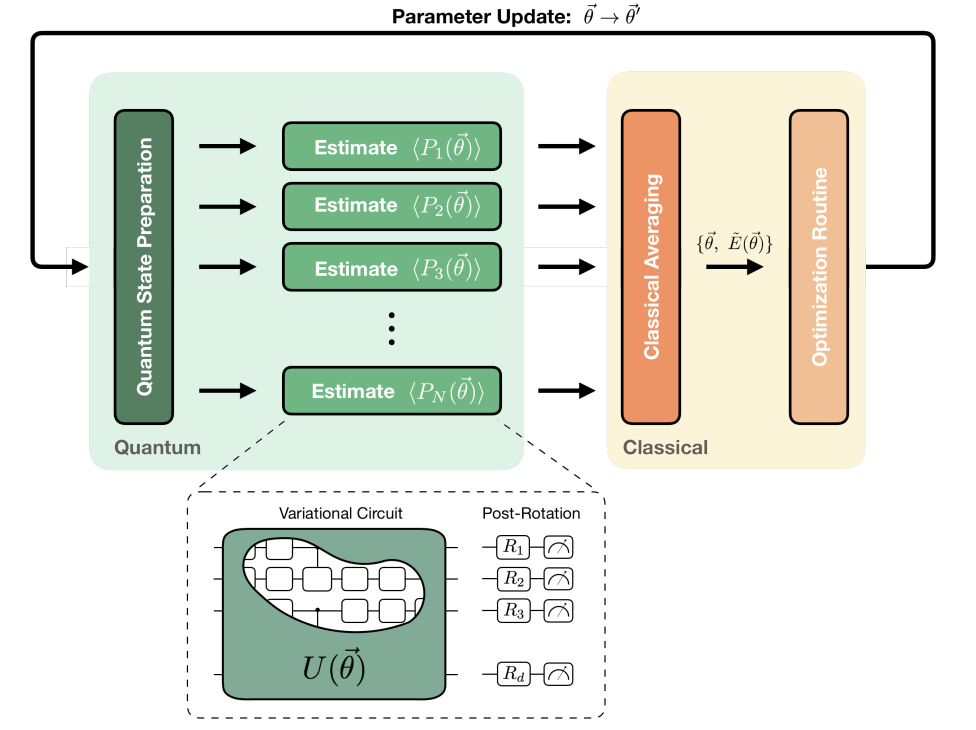
\includegraphics[width=\linewidth]{VQE_precedure.png}
      \caption{Taken from:\cite{Cao2019}; Illustration of the VQE algorithm. the quantum computer is used to prepare a set of parametrized quantum states followed by applications of rotations $R_i$. The classical computer then takes the individual estimates of the Pauli term expectation values $<P_i(\stackrel{\rightarrow}{\theta})>$ and averages them to compute a single value $\overline{E}(\stackrel{\rightarrow}{\theta})$. This cost function value is fed into an optimization routine, which produces an updated set of parameters $\stackrel{\rightarrow}{\theta}$ as input for the quantum circuit in the next optimization loop. This procedure is repeated until the energy converges.}
      \label{fig:VQE} 
  \end{figure}
\end{center}

Using the optimal parameter values $\theta^*\equiv \text{argmin}_{\theta}\langle \hat{\text{H}} \rangle_{U(\theta)}$, one can write the ground state of the system as $|\Psi\rangle=U(\theta^*)|0\rangle$. When using a UCC-type ansatz the HF reference state has to be contained in $U(\theta)$.

\subsection{The k-UpCCGSD Ansatz}

The k-UpCCGSD (k Pair Unitary Coupled Cluster with Generalized Singles and Doubles) ansatz introduced in "Generalized Unitary Coupled Cluster Wavefunctions for Quantum Computation" \cite{Lee2019} encorporates aspects of multiple CC variations as a way of obtaining an accurate and computationally efficient ansatz.

In Generalized CC (GCC) the single and double excitation terms do not distinguish between occupied and unoccupied orbitals, and are therefore referred to as generalized singles and doubles (GSD). As a result CCGSD allows for excitations from occupied to virtual orbitals, as well as excitations from occupied to occupied ones, which yields a more accurate and robust ansatz when compared to the simpler UCCSD.

pCCD \cite{Stein2014}, also known as Ap1roG \cite{Limacher2013} is a variation on CC which a very limited number of doubles amplitudes, namely it contains only the two body excitations that move a pair of electrons from one spatial orbital to another:

\begin{align}
\hat{T}_2=\sum_{ia}t_{i_{\alpha}i_{\beta}}^{a_{\alpha}a_{\beta}}\hat{a}_{a_{\alpha}}^{\dagger}\hat{a}_{a_{\beta}}^{\dagger}\hat{a}_{i_{\beta}}\hat{a}_{i_{\alpha}}
\end{align}

where the summation runs over occupied and unoccupied spatial orbitals.

Despite being much simpler than spin-restricted CCSD (RCCSD) pCCD is less prone to a non-variational failure when breaking bonds.

The k-UpCCGSD model uses generalized singles and pair Doubles, and takes a product of a total of k unitary operators to increase the flexibility of the wavefunction. For a chosen integer k, k-UpCCGSD is defined as:

\begin{align}
|\Psi\rangle=\prod_{\alpha=1}^{k}(e^{\hat{T}^{(\alpha)}-\hat{T}^{(\alpha)\dagger}})|\Phi_{\text{ref}}\rangle
\end{align}

where each $\hat{T}^{(\alpha)}$ contains its own independent set of variational parameters $\theta$. Because the doubles term in k-UpCCGSD is so limited when compared to standard UCCSD, its circuit depth is greatly decreased and scales linearly with system size, with a prefactor that is increased by a factor of k.

\subsection{Summary of the Quantum UCC procedure}

To create the UCC ansatz and optimize the $\theta$ parameters in a VQE procedure, these steps can be followed:

\begin{itemize}
  \item Defining the molecular system of interest by providing the atoms, their coordinates and the basis set.
  \item Mapping the electronic structure problem onto a quantum circuit using transforms such as Jordan-Wigner.
  \item Constructing the UCC ansatz.
  \item Defining the objective function (the expectation value of the Hamiltonian operator with respect to the UCC ansatz).
  \item choosing an optimization algorithm such as VQE.
  \item (optionally choosing a backend for simulating quantum hardware)
  \item Performing the VQE optimization to find the optimal parameters (\cref{fig:VQE}).
  \item Computing the final energy.
\end{itemize}

\section{Methodology}

The UCC ansätze evaluated in ensuing parts of this outline were constructed in python using the \href{https://qiskit.org/}{qiskit} library for working with quantum computers. The VQE algorithm was likewise sourced from qiskit. The orbitals represented in quantum circuits by qubits were obtained using the STO-3G basis set, as it is a minimalistic molecular system that can be easily represented using a small number of qubits. Moreover STO-3G can be used as a standardized benchmark, making it possible for different research groups and quantum computing platforms to compare their results and methodologies on a common test case. Likewise the FCI, classical CC, and HF calculations, which quantum UCC calculations were compared to, were also performed using the STO-3G basis set. It's worth noting that qiskit by default associates the qubits in generated circuits first with alpha orbitals, followed by beta orbitals. This has to be kept in mind while constructing ansätze, as some circuits may at face value appear different then the ones presented in this outline. The dissociation curve calculated using a noisy backend simulation was generated using \href{https://github.com/tequilahub/tequila}{tequila}, as it provides a much more flexible environment for chemical computations when compared to qiskit.

\section{Results and discussion}

\cref{fig:H2} presents the dissociation curve of $\text{H}_2$ obtained on an ideal quantum backend (no noise) using quantum UCCS and pUCCD ansätze with classical pCCD, HF, and FCI references. UCCS matches the energies obtained from HF, which means that UCCS relies on the HF reference state embedded within the ansatz. On the other hand UpCCD is able to match FCI and classical pCCD results.

\begin{center}
  \begin{figure}[h]
      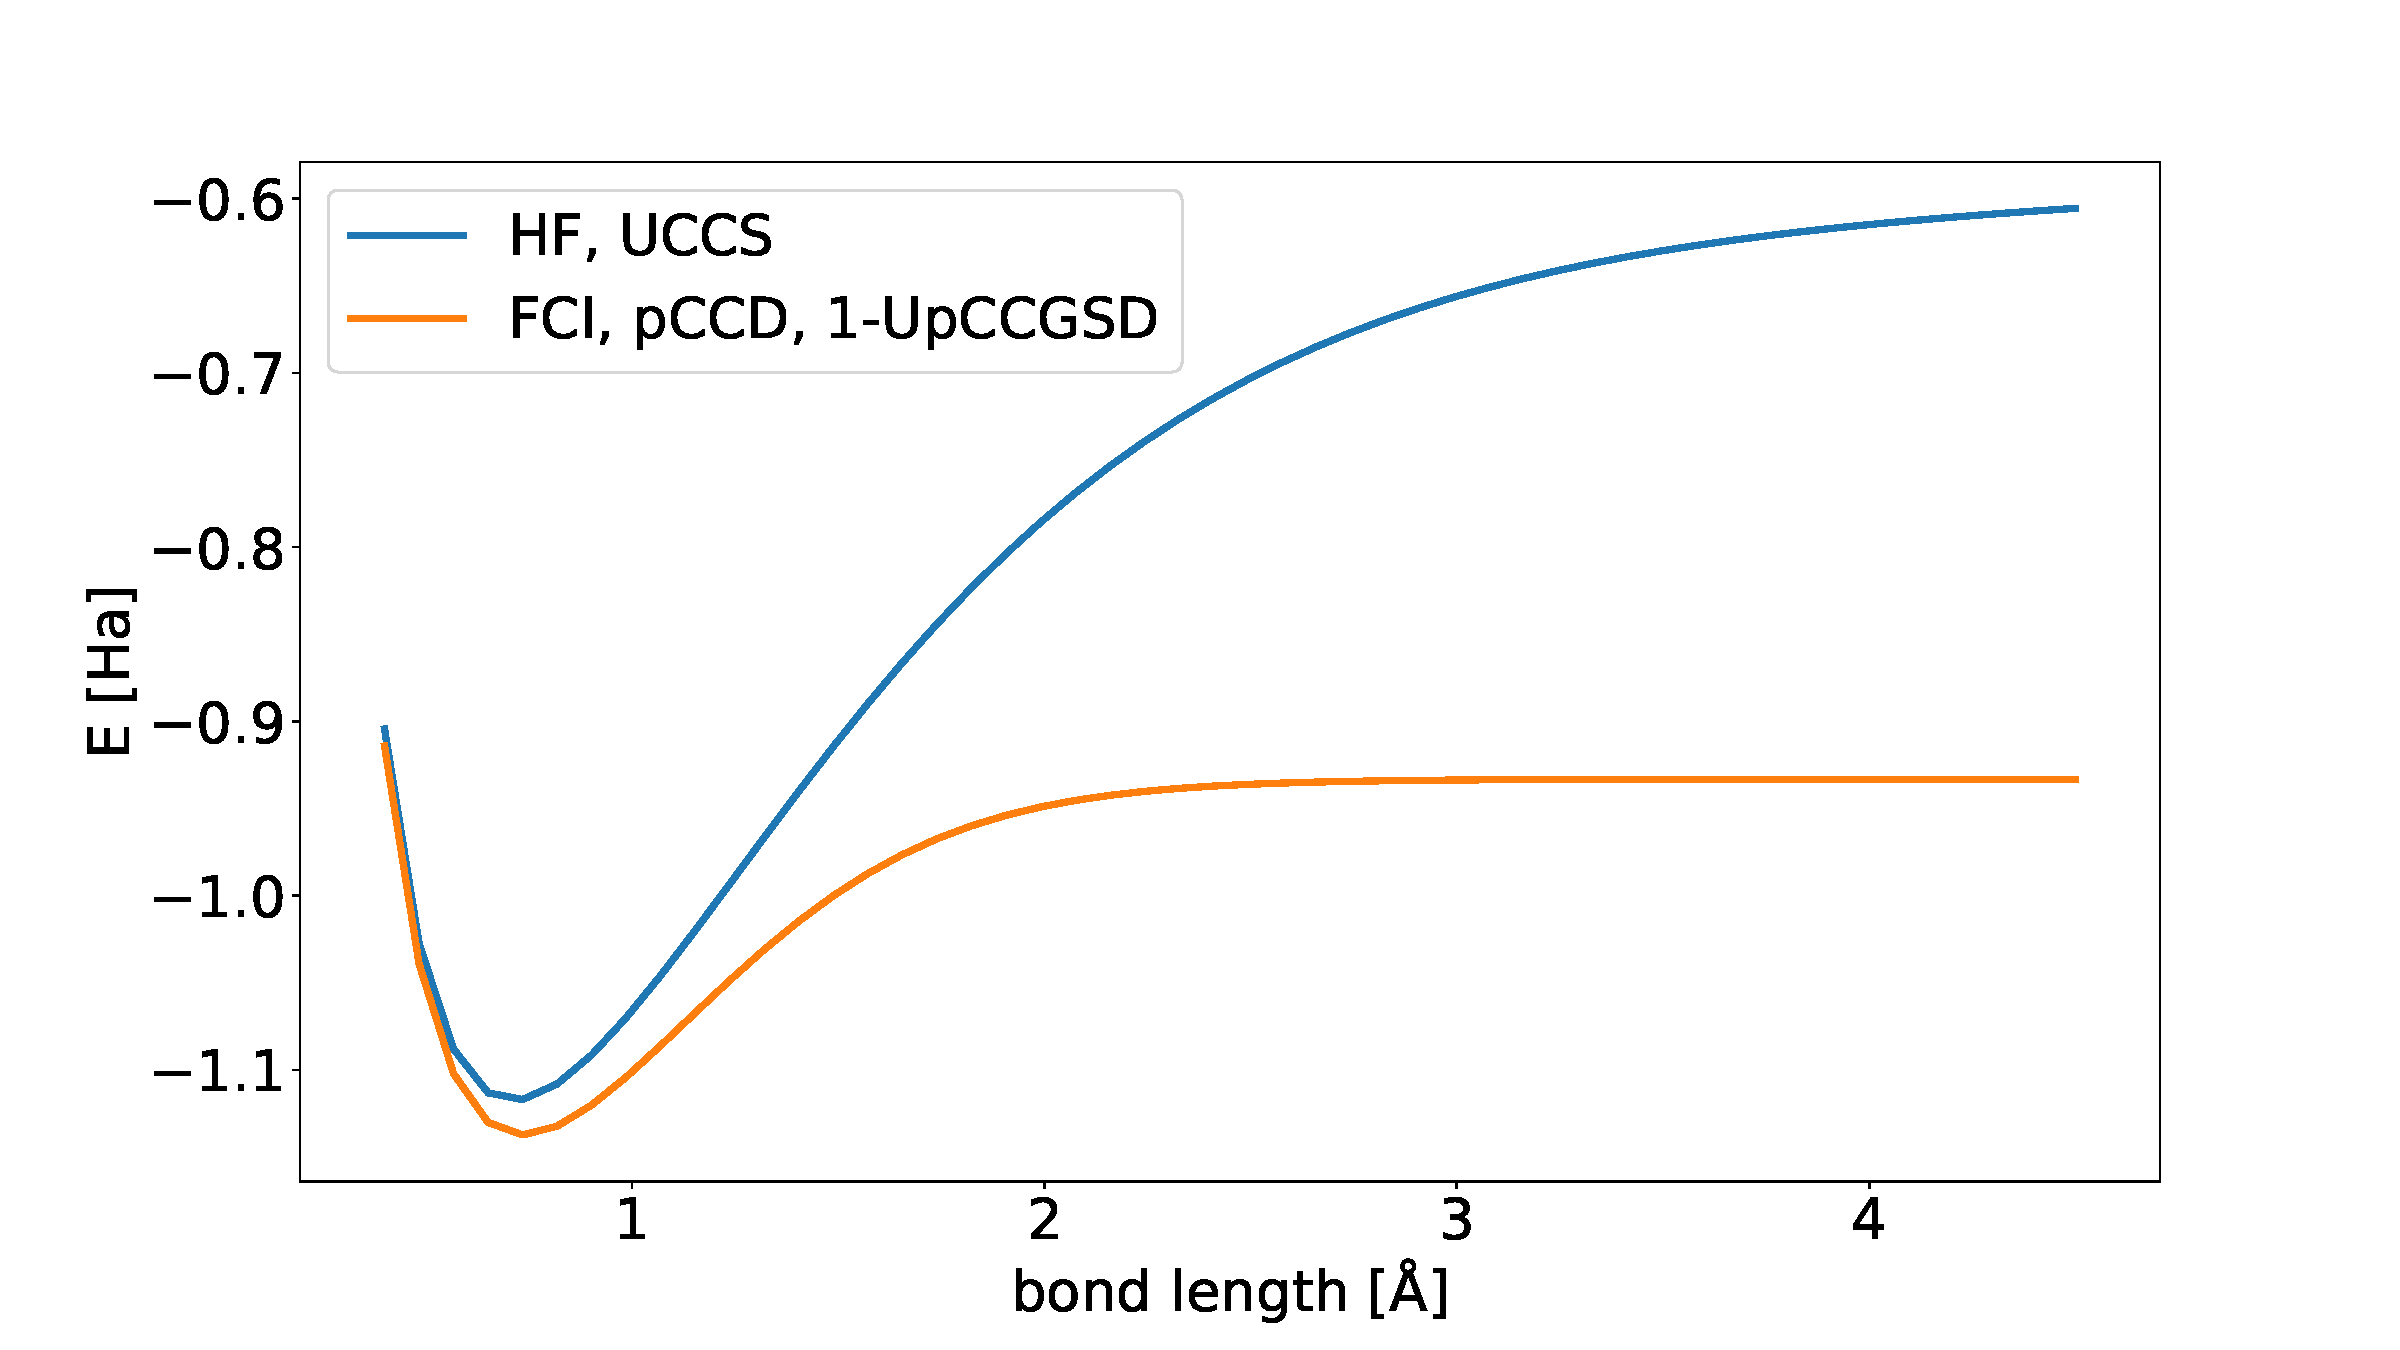
\includegraphics[width=\linewidth]{QC_UCC_HH.pdf}
      \caption{Dissociation curve of $\text{H}_2$ for FCI, HF and classical pCCD, as well as UCCS, UpCCD evaluated on an ideal noise-free backend.}
      \label{fig:H2} 
  \end{figure}
\end{center}

However current quantum computers are far from ideal devices, \cref{fig:H2_noisy} presents a more accurate representation of current quantum hardware capabilities. The simulator used in this calculation was the "Rome" device simulator from qiskit, a 5 qubit simulation backend that emulates the behavior of a quantum device known as the IBM Quantum Rome. The Rome device simulator in qiskit aims to mimic the noise and error characteristics of the IBM Quantum Rome device, including features such as gate errors, measurement errors, and various noise sources that are present in real quantum hardware.

\begin{center}
  \begin{figure}[h]
      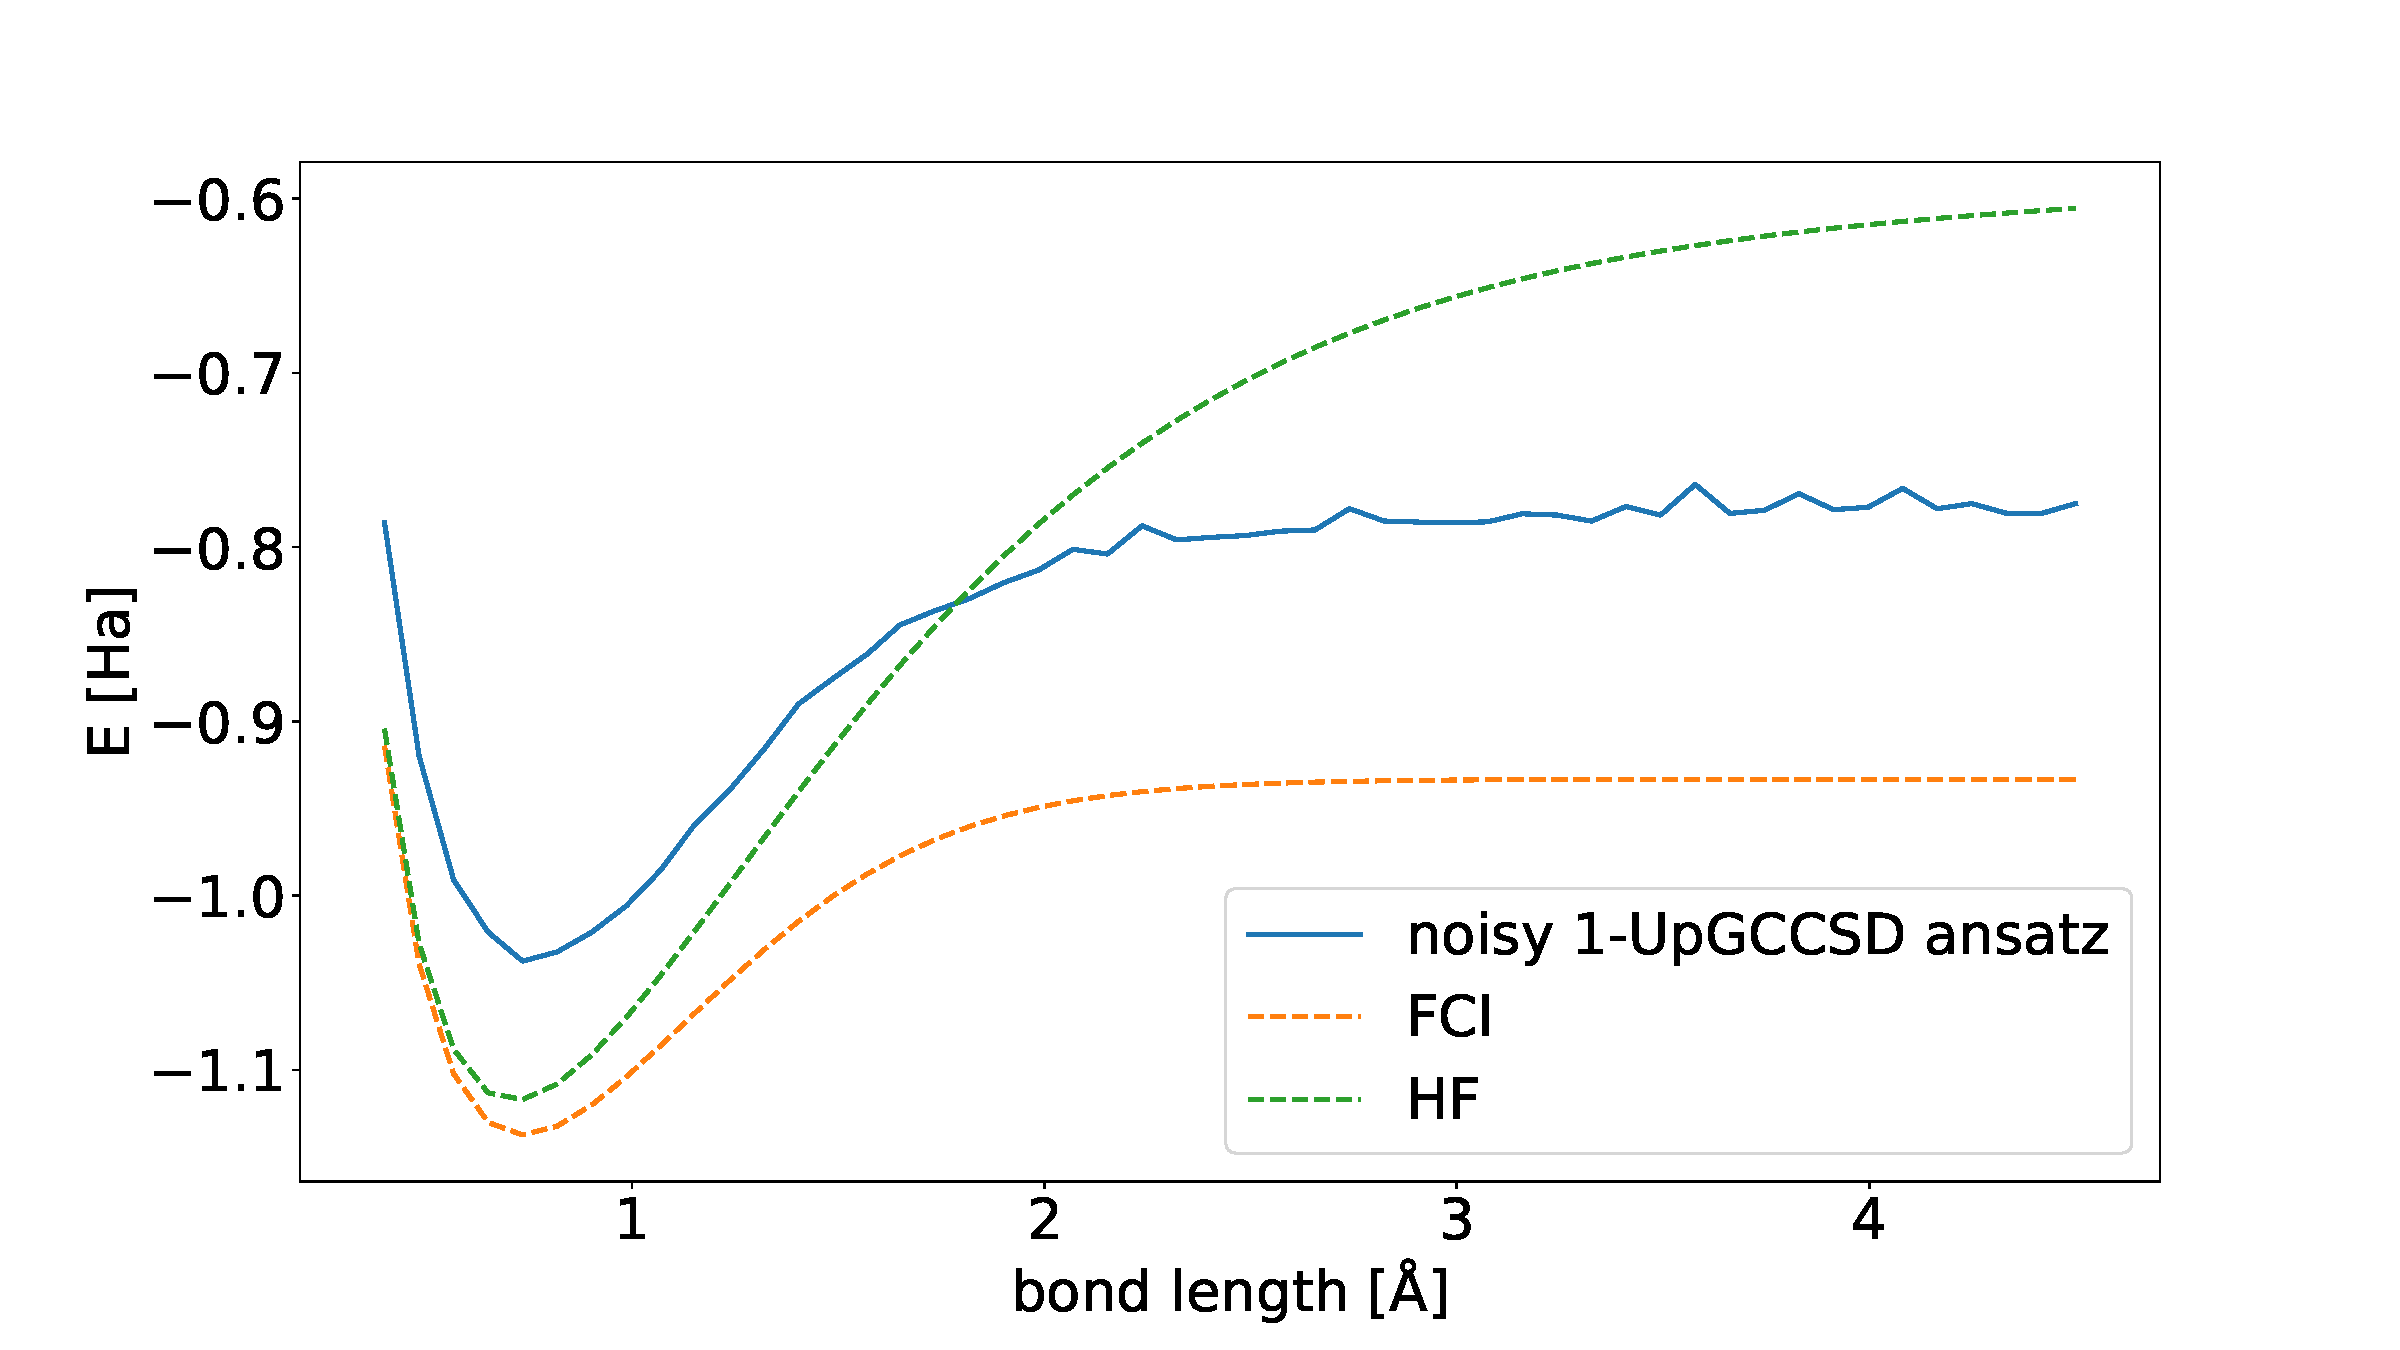
\includegraphics[width=\linewidth]{QC_UCC_HH_noisy.pdf}
      \caption{Dissociation curve of $\text{H}_2$ for FCI, HF, and UpCCD evaluated on a noisy backend.}
      \label{fig:H2_noisy} 
  \end{figure}
\end{center}

\section{Conclusions}

In theory, integrating quantum computing with an already powerful method such as Coupled Cluster has the potential to open up a number of new avenues within the field of quantum chemistry, and greatly enhance our capabilities to model molecular systems. However, this prospect is held back by the current state of quantum hardware, which to this day remains in a rather rudimentary stage of development. Modern quantum computers are unreliable and don't offer any significant advantages over their classical counterparts. Because of this the future of quantum implementations of Unitary Coupled Cluster remains closely tied to any potential advancements made in the realm of quantum computing. However, even with the current hardware limitations, there is still an incentive to improve both the theoretical and practical accuracy and efficiency of quantum UCC ansätze.

\section*{Appendix}
    % \begin{tikzpicture}[thick]
    % % `operator' will only be used by Hadamard (H) gates here.
    % % `phase' is used for controlled phase gates (dots).
    % % `surround' is used for the background box.
    % \tikzstyle{operator} = [draw,fill=white,minimum size=1.5em] 
    % \tikzstyle{phase} = [draw,fill,shape=circle,minimum size=5pt,inner sep=0pt]
    % \tikzstyle{not} = [font=\bfseries,draw,shape=circle,minimum size=5pt,inner sep=0pt]
    % \tikzstyle{surround} = [fill=blue!15,thick,draw=black,rounded corners=2mm,inner ysep=7pt]
    % %
    % \matrix[row sep=0.4cm, column sep=0.2cm] (circuit) {
    % % First row.
    % \node (q1) {$q_0$}; &&
    % \node[operator] (R11) {$\text{R}_{\text{x}}(\frac{\pi}{2})$}; &
    % \node[phase] (P12) {}; &
    % &
    % \node[phase] (P14) {}; &
    % \node[operator] (R15) {$\text{R}_{\text{x}}(-\frac{\pi}{2})$}; &
    % \node[operator] (H16) {H}; &
    % \node[phase] (P17) {}; &&
    % \node[phase] (P18) {}; &
    % \node[operator] (H19) {H}; &
    % \coordinate (end1); \\
    % % Second row.
    % \node (q2) {$q_1$}; &&
    % \node[operator] (H21) {H}; &
    % \node[not] (P22) {|}; &
    % \node[operator] (R23) {$\text{R}_{\text{z}}(\theta)$}; &
    % \node[not] (P24) {|}; &
    % \node[operator] (H25) {H}; &
    % \node[operator] (R26) {$\text{R}_{\text{x}}(\frac{\pi}{2})$}; &
    % \node[not] (P27) {|}; &
    % \node[operator] (R28) {$\text{R}_{\text{z}}(-\theta)$}; &
    % \node[not] (P29) {|}; &
    % \node[operator] (R291) {$\text{R}_{\text{x}}(-\frac{\pi}{2})$}; &
    % \coordinate (end2);\\
    % };
    % \begin{pgfonlayer}{background}
    %     % Draw background box.
    %     \node[surround] (background) [fit = (q1) (H21) (end2)] {};
    %     % Draw lines.
    %     \draw[thick] (q1) -- (end1)  (q2) -- (end2) (P12) -- (P22) (P14) -- (P24) (P17) -- (P27) (P18) -- (P29);
    % \end{pgfonlayer}
    % %
    % \end{tikzpicture}\\
    \begin{center}
    \begin{figure}[h]
      \begin{tikzpicture}[thick]
        \tikzstyle{operator} = [draw,fill=white,minimum size=1.5em] 
        \tikzstyle{phase} = [draw,fill,shape=circle,minimum size=5pt,inner sep=0pt]
        \tikzstyle{not} = [font=\bfseries,draw,shape=circle,minimum size=5pt,inner sep=0pt]
        \tikzstyle{surround} = [fill=blue!15,thick,draw=black,rounded corners=2mm,inner ysep=7pt]
        %
        \matrix[row sep=0.4cm, column sep=0.2cm] (circuit) {
        % First row.
        \node (q1) {$q_p$}; &&
        \node[operator] (R11) {H}; &
        \node[phase] (P12) {}; &
        &&&&&
        \node[phase] (P14) {}; &
        \node[operator] (R15) {H}; &
        \node[operator] (H16) {$\text{R}_{\text{x}}(\frac{\pi}{2})$}; &
        \node[phase] (P17) {}; &&&&&&&
        \node[phase] (P18) {}; &
        \node[operator] (H19) {$\text{R}_{\text{x}}(-\frac{\pi}{2})$}; &
        \coordinate (end1); \\
        % Second row
        \node (q2) {$q_{p+1}$}; &&
        &
        \node[not] (P22) {|}; &
        \node[phase] (P23) {}; &
        &&&
        \node[phase] (P24) {}; &
        \node[not] (P25) {|}; &&&
        \node[not] (P26) {|}; &
        \node[phase] (P27) {}; &&&&
        \node[phase] (P28) {}; &&
        \node[not] (P29) {|}; &&
        \coordinate (end2); \\
        % Third row
        \node (q3) {$q_{k-1}$}; &&
        &&
        \node[not] (P32) {|}; &
        \node[phase] (P33) {}; &
        &
        \node[phase] (P34) {}; &
        \node[not] (P35) {|}; &&&&&
        \node[not] (P36) {|}; &
        \node[phase] (P37) {}; &&
        \node[phase] (P38) {}; &
        \node[not] (P39) {|}; &&&&
        \coordinate (end3); \\
        % Fourth row.
        \node (q4) {$q_k$}; &&
        \node[operator] (H41) {$\text{R}_{\text{x}}(\frac{\pi}{2})$}; &&&
        \node[not] (P42) {|}; &
        \node[operator] (R43) {$\text{R}_{\text{z}}(\theta)$}; &
        \node[not] (P44) {|}; &&&
        \node[operator] (H45) {$\text{R}_{\text{x}}(-\frac{\pi}{2})$}; &
        \node[operator] (R46) {H}; &&&
        \node[not] (P47) {|}; &
        \node[operator] (R48) {$\text{R}_{\text{z}}(-\theta)$}; &
        \node[not] (P49) {|}; &&&&
        \node[operator] (R46) {H}; &
        \coordinate (end4);\\
        };
        \begin{pgfonlayer}{background}
            % Draw background box.
            \node[surround] (background) [fit = (q1) (H41) (end4)] {};
            % Draw lines.
            \draw[thick] (q1) -- (end1) (q2) -- (end2) (q3) -- (end3) (q4) -- (end4) (P12) -- (P22) (P33) -- (P42) (P14) -- (P25) (P34) -- (P44) (P17) -- (P26) (P37) -- (P47) (P38) -- (P49) (P18) -- (P29);
            \node at ($(q2)!.35!(q3)$) {\vdots};
            \node at ($(P23)!.35!(P32)$) {\vdots};
            \node at ($(P24)!.35!(P35)$) {\vdots};
            \node at ($(P27)!.35!(P36)$) {\vdots};
            \node at ($(P28)!.35!(P39)$) {\vdots};
        \end{pgfonlayer}
        %
        \end{tikzpicture}
    \caption{The full circuit for a single fermionic excitation denoted by:\\ $U_p^k(\theta)=e^{-i\frac{\theta}{2}(X_pY_k-Y_pX_k)\prod_{r=p+1}^{k-1}Z_r}$.}
    \label{fig:full single}
  \end{figure}
\end{center}
    % \begin{tikzpicture}[thick]
    %   \tikzstyle{operator} = [draw,fill=white,minimum size=1.5em] 
    %   \tikzstyle{phase} = [draw,fill,shape=circle,minimum size=5pt,inner sep=0pt]
    %   \tikzstyle{not} = [font=\bfseries,draw,shape=circle,minimum size=5pt,inner sep=0pt]
    %   \tikzstyle{surround} = [fill=blue!15,thick,draw=black,rounded corners=2mm,inner ysep=7pt]
    %   %
    %   \matrix[row sep=0.4cm, column sep=0.2cm] (circuit) {
    %   % First row.
    %   \node (q1) {$q_k$}; &&
    %   \node[operator] (H11) {H}; &

    %   \node[phase] (P12) {}; &&&&&&
    %   \node[phase] (P13) {}; &

    %   \node[operator] (H14) {H}; &
      
    %   \coordinate (end1); &&&
    %   \coordinate (end10);\\

    %   % Second row
    %   \node (q2) {$q_l$}; &&
    %   \node[operator] (H21) {H}; &

    %   \node[not] (P22) {|}; &
    %   \node[phase] (P23) {}; &&&&
    %   \node[phase] (P24) {}; &
    %   \node[not] (P25) {|}; &

    %   \node[operator] (H26) {H}; &
            
    %   \coordinate (end2); &&&
    %   \coordinate (end20);\\

    %   % Third row
    %   \node (q3) {$q_j$}; &&
    %   \node[operator] (R31) {$\text{R}_{\text{x}}(\frac{\pi}{2})$}; &&

    %   \node[not] (P32) {|}; &
    %   \node[phase] (P34) {}; &&
    %   \node[phase] (P35) {}; &
    %   \node[not] (P36) {|}; &&

    %   \node[operator] (R37) {$\text{R}_{\text{x}}(-\frac{\pi}{2})$}; &
      
    %   \coordinate (end3); &&&
    %   \coordinate (end30);\\

    %   % Fourth row.
    %   \node (q4) {$q_i$}; &&
    %   \node[operator] (H41) {H}; &&&

    %   \node[not] (P42) {|}; &

    %   \node[operator] (R43) {$\text{R}_{\text{z}}(\theta)$}; &

    %   \node[not] (P44) {|}; &&&

    %   \node[operator] (H45) {H}; &
      
    %   \coordinate (end4); &&&
    %   \coordinate (end40);\\
    %   };
    %   \begin{pgfonlayer}{background}
    %       % Draw background box.
    %       \node[surround] (background) [fit = (q1) (H41) (end40)] {};
    %       % Draw lines.
    %       \draw[thick] (q1) -- (end1) (q2) -- (end2) (q3) -- (end3) (q4) -- (end4) (P12) -- (P22) (P34) -- (P42) (P35) -- (P44) (P13) -- (P25);

    %       \node at ($(q2)!.35!(q3)$) {\vdots};
    %       \node at ($(P23)!.35!(P32)$) {\vdots};
    %       \node at ($(P24)!.35!(P36)$) {\vdots};
    %       \node at ($(end4)!.5!(end40)$) {\ldots};
    %       \node at ($(end1)!.5!(end10)$) {\ldots};
    %       \node at ($(end2)!.5!(end20)$) {\ldots};
    %       \node at ($(end3)!.5!(end30)$) {\ldots};
    %   \end{pgfonlayer}
    %   %
    %   \end{tikzpicture}\\

%%%END OF MAIN TEXT%%%

%The \balance command can be used to balance the columns on the final page if desired. It should be placed anywhere within the first column of the last page.

\balance

%If notes are included in your references you can change the title from 'References' to 'Notes and references' using the following command:
%\renewcommand\refname{Notes and references}

\newpage

%%%REFERENCES%%%
\bibliography{outline} %You need to replace "rsc" on this line with the name of your .bib file
\bibliographystyle{aip} %the AIP's .bst file

\end{document}